





\section{music}
fq{“Much of what was in Doom Bible never appeared in the game, but it set a mood for starting on the project. Within a few months of receiving that document, I had roughed out a lot of music and most of what turned out to be final sound effects.”}{Bobby Prince, Retro Gamer 44.}

\fq{The id Software development team originally wanted me to do nothing but metal songs for DOOM. I did not think that this type of music would be appropriate throughout the game, but I roughed out several original songs and also created MIDI sequences of some cover material. This was before any level design and was before most of the artwork had been created. As the game came together, the guys at id saw that this type of music was not appropriate for many of the levels in DOOM. Thinking that this would be the case, I had also roughed out a lot of ambient moody background music, much of which ended up in the game. This song ("At Doom's Gate") was one of the first of its type that I wrote. I heard it as being on a level that went by real fast. As it turns out, John Romero (who placed all of the songs on the levels) decided it was a perfect song for the first level.}{Bobby}

\section{audio samples}

"Body Movin" music video features the door song at the 5:09 mark.\\
\par
imp dying sound is a camel.\\
\par
Source: Commercial sound library created by Sound Ideas\\
\par
In a baffling move, Doom (2005), the film did not tap into those now-famous Sound Ideas effects. except for the scene that most folks deem to be the best in the film.\\
\trivia{DMXGUS contains a TEXT FILE with comments...}

\section{Distribution}
\fq{We don’t care if you make money off this shareware demo,” Jay told retailers. “Move it. Move it in mass quantities.” The retailers couldn’t believe their ears, no one had ever told them not to pay royalties.
But Jay was insistent. “Take DOOM for nothing, keep the profit. My goal is distribution. DOOM is going to
be Wolfenstein on steroids, and I want it far and wide.
I want you to stack DOOM high. In fact, I want you to
do advertising for it, too, because you’re going to make money off it. So take this money that you might have given me in royalties and use it to advertise the fact that you’re selling DOOM.}{Jay}


\section{Dave Taylor Leak anecdote}




\section{Credit Screen Evolution}

\trivia{The credit screen evolved with each beta version of Doom. Notice how NeXT computer were originally credited, witnessing how important the development machine were to id. In version 1.25, Michael Abrash (who would only join id for Quake) was credited due to the quality of his article in XXX and Graphic Black Book ???.}\\
\par
\cscaledimage{0.92}{credits/DoomCREDIT10.png}{v1.0}
\par
\cscaledimage{0.92}{credits/DoomCREDIT19.png}{v1.1 to v1.9}
\par
\cscaledimage{0.92}{credits/DoomCREDIT125.png}{v1.25}
\par
\cscaledimage{0.92}{credits/DoomCREDITUD.png}{Ultimate Doom}
\par

\pagebreak
\section{Programming}
Migrating from Borland C++ editor on DOS to TextEdit on NeXT Step was a bittersweet experience. On one side convenient things such as syntax highlighting were lost. On the other side, the machine never crashes and developers never had to curse over hours lost. The high resolution (1120 x 832) allowed to see full function vertically and three DOS windows horizontally. \\
\par
\fullimage{development.png}
\par
\fullimage{TextEditApp.png}
\begin{figure}[H]
\centering
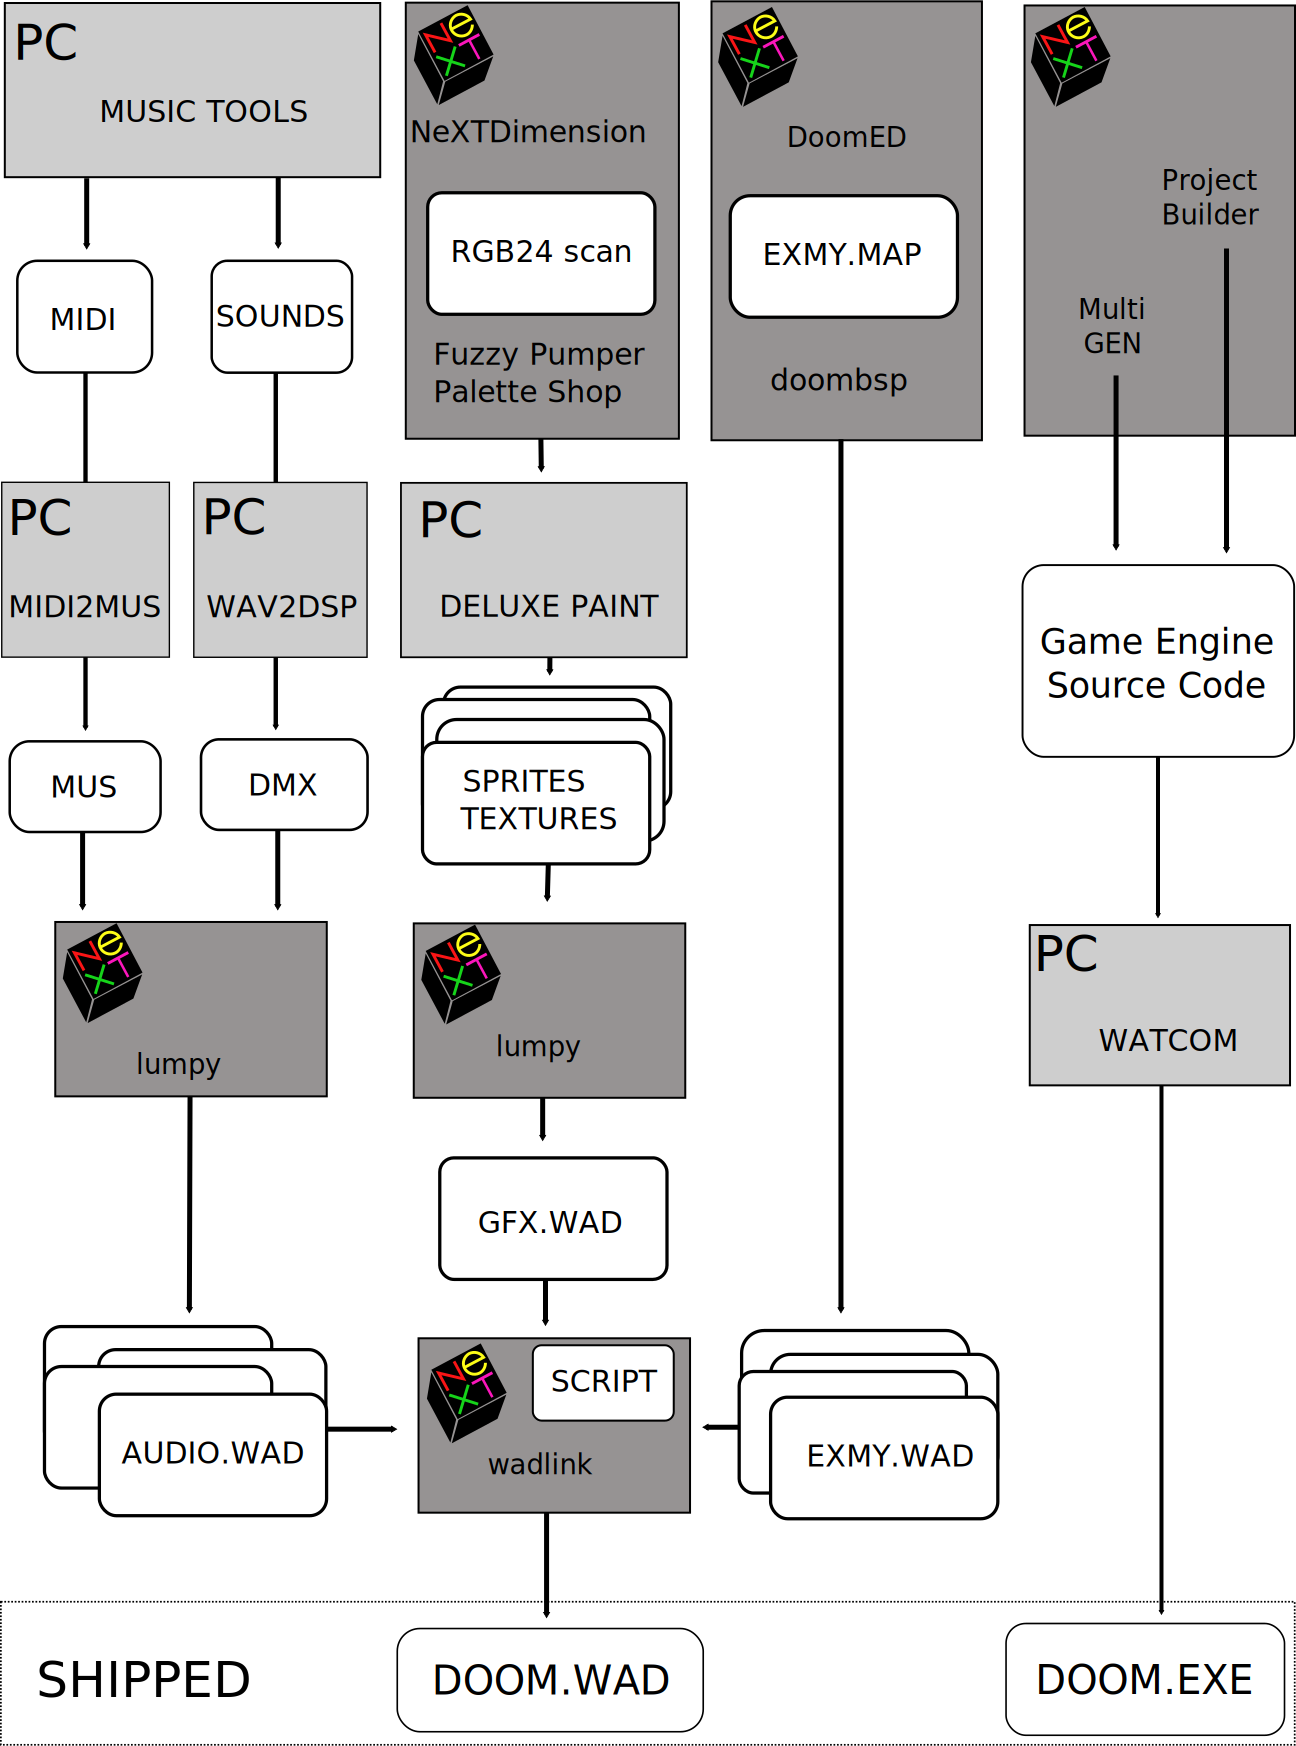
\includegraphics[width=\textwidth]{drawings/doom_pipeline.pdf}
\caption{Doom assets pipeline.}
\end{figure}
\par

\section{doombsp}
\cfullimage{doombsp_compiling.png}{}
\par
\cfullimage{doombsp_run.png}{}
\par



\section{Sound effects}
bla
\section{Musics}
bla


\section{TO DELETE MAYBE}
\par
\fullimage{bestiary.png}
TODO: TABLE SUMMARIZING HOW ASSETS WERE DONE.\\
\trivia{Gregor is the son of Don Ivan Punchatz, who created the Doom package art and logo.}\\
